%! TEX program = xelatex
% Paquetes:
\documentclass[letterpaper, 12pt]{article}
\usepackage[spanish]{babel} %%Paquete español para mac
\usepackage{graphicx} %% Para incluir figuras
\usepackage{xcolor}
\usepackage{ifpdf}
\usepackage{circledsteps}
\DeclareGraphicsExtensions{.pdf}
\usepackage[margin=1in]{geometry}
\setcounter{totalnumber}{5}
\renewcommand{\textfraction}{0.1}
\usepackage[cmex10]{amsmath}
\usepackage{amssymb}
\usepackage{float}
\usepackage{cite}
\bibliographystyle{unsrt}
%\decimalpoint
\usepackage{url}
\usepackage{hyperref}
\hypersetup{colorlinks=false,bookmarksopen=true,linkbordercolor={1 1 1}}
%\usepackage{epstopdf}
\usepackage{mathtools}
\usepackage{chngcntr}
\usepackage{enumitem}
\providecommand{\e}[1]{\ensuremath{\times 10^{#1}}}
\usepackage[parfill]{parskip} % Líneas en lugar de indentación
\usepackage{fancyhdr}
\usepackage{booktabs}
\usepackage{cleveref}
\usepackage{verbatimbox}
\crefformat{footnote}{#2\footnotemark[#1]#3}

\usepackage[squaren]{SIunits} %esto me da nombres de unidades y prefijos
\usepackage{sistyle}% Esto es adecuado para escribir unidades.

\newcommand{\alumno}{Agustín Campeny}
\lhead{\nouppercase{\leftmark}}
\rhead{Tarea 3 - \alumno}
\pagestyle{fancy}
%\usepackage{scrextend}
\numberwithin{equation}{section}

\setlength{\tabcolsep}{6pt} % General space between cols (6pt standard)
\renewcommand{\arraystretch}{0.8} % General space between rows (1 standard)
\begin{document}
\thispagestyle{empty}
%%%%%%%%%%%%%%%%%%%%%%%%%%
%%%%%%%%% ENCABEZADO %%%%%%%%%
%%%%%%%%%%%%%%%%%%%%%%%%%%
\vspace*{-1cm}

\includegraphics[width=2cm]{logo.pdf}
\vspace*{-2.2cm}

\hspace*{2cm}
 \begin{tabular}{l}
  {\ \textsc{\raggedright \footnotesize Pontificia Universidad Católica de Chile}}\\
  {\ \textsc{\raggedright \footnotesize Escuela de Ingeniería}}\\
  {\ \textsc{\raggedright \footnotesize Departamento de Ingeniería Eléctrica}}\\
  {\ \textsc{\raggedright \footnotesize IEE2753 - Diseño de Circuitos Integrados Digitales}}\\
  {\  }\\
 \end{tabular}
 \hfill
\vspace*{-0.2cm}
\begin{center}
  {\Large\bf Tarea 3}\\
\vspace*{2mm}
{\today}\\
\vspace*{2mm}
{\footnotesize \alumno}\\
\vspace*{6mm}
\end{center}
\hrule\vspace*{2pt}\hrule
%%%%%%%%%%%%%%%%%%%%%%%%%%
%%%%%%%%% ENCABEZADO %%%%%
%%%%%%%%%%%%%%%%%%%%%%%%%%

\section{Intento de buffer}

\begin{enumerate}[label=\Alph*.]

  \item Se presenta un bosquejo de la curva de transferencia del circuito.

    \begin{figure}[H]
      \centering
      % XCircuit output "/Users/agustincampenyscolari/Desktop/IEE2753/IEE2753-2020-agustincampeny/tarea3/report/p1_1.tex" for LaTeX input from /Users/agustincampenyscolari/Desktop/IEE2753/IEE2753-2020-agustincampeny/tarea3/report/p1_1.eps
\def\putbox#1#2#3#4{\makebox[0in][l]{\makebox[#1][l]{}\raisebox{\baselineskip}[0in][0in]{\raisebox{#2}[0in][0in]{\scalebox{#3}{#4}}}}}
\def\rightbox#1{\makebox[0in][r]{#1}}
\def\centbox#1{\makebox[0in]{#1}}
\def\topbox#1{\raisebox{-0.60\baselineskip}[0in][0in]{#1}}
\def\midbox#1{\raisebox{-0.20\baselineskip}[0in][0in]{#1}}
   \scalebox{1}{
   \normalsize
   \parbox{4.6875in}{
   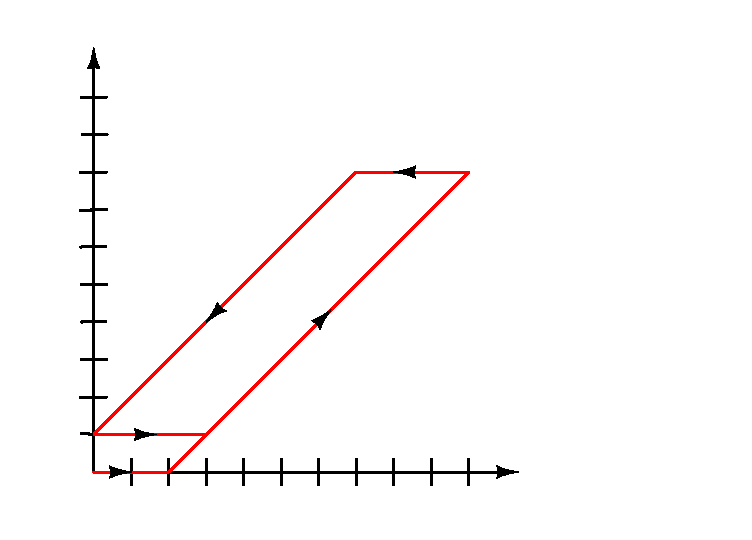
\includegraphics[scale=1]{/Users/agustincampenyscolari/Desktop/IEE2753/IEE2753-2020-agustincampeny/tarea3/report/p1_1.eps}\\
   % translate x=632 y=503 scale 0.38
   \putbox{3.35in}{0.18in}{1.20}{$V_{\text{in}}$}%
   \putbox{0.10in}{3.18in}{1.20}{$V_{\text{out}}$}%
   \putbox{0.89in}{0.09in}{1.20}{0.2}%
   \putbox{1.39in}{0.09in}{1.20}{0.4}%
   \putbox{1.89in}{0.09in}{1.20}{0.6}%
   \putbox{2.39in}{0.09in}{1.20}{0.8}%
   \putbox{2.89in}{0.09in}{1.20}{$V_{DD}$}%
   \putbox{0.14in}{0.76in}{1.20}{0.2}%
   \putbox{0.14in}{1.26in}{1.20}{0.4}%
   \putbox{0.14in}{1.76in}{1.20}{0.6}%
   \putbox{0.14in}{2.26in}{1.20}{0.8}%
   \putbox{0.06in}{2.80in}{1.20}{$V_{DD}$}%
   \putbox{0.43in}{0.09in}{1.20}{\Circled{1}}%
   \putbox{2.18in}{1.34in}{1.20}{\Circled{2}}%
   \putbox{2.51in}{2.43in}{1.20}{\Circled{3}}%
   \putbox{1.43in}{1.34in}{1.20}{\Circled{4}}%
   \putbox{0.76in}{0.68in}{1.20}{\Circled{5}}%
   } % close 'parbox'
   } % close 'scalebox'
   \vspace{-\baselineskip} % this is not necessary, but looks better

      \caption{Bosquejo de la curva de transferencia del circuito}
    \end{figure}

Se pueden notar 5 estados diferentes:

\begin{enumerate}[label=\protect\Circled{\arabic*}]

  \item Ambos transistores en corte.

  \item NMOS en región de saturación, PMOS en corte.

  \item Ambos transistores en corte.

  \item PMOS en región de saturación, NMOS en corte.

  \item Ambos transistores en corte.

\end{enumerate}

\item Se presenta un gráfico con las formas de onda correspondientes a \(V_{\text{in}}\) y \(V_{\text{out}}\):

    \begin{figure}[H]
      \centering
      % XCircuit output "/Users/agustincampenyscolari/Desktop/IEE2753/IEE2753-2020-agustincampeny/tarea3/report/p1_2.tex" for LaTeX input from /Users/agustincampenyscolari/Desktop/IEE2753/IEE2753-2020-agustincampeny/tarea3/report/p1_2.eps
\def\putbox#1#2#3#4{\makebox[0in][l]{\makebox[#1][l]{}\raisebox{\baselineskip}[0in][0in]{\raisebox{#2}[0in][0in]{\scalebox{#3}{#4}}}}}
\def\rightbox#1{\makebox[0in][r]{#1}}
\def\centbox#1{\makebox[0in]{#1}}
\def\topbox#1{\raisebox{-0.60\baselineskip}[0in][0in]{#1}}
\def\midbox#1{\raisebox{-0.20\baselineskip}[0in][0in]{#1}}
   \scalebox{1}{
   \normalsize
   \parbox{5.56771in}{
   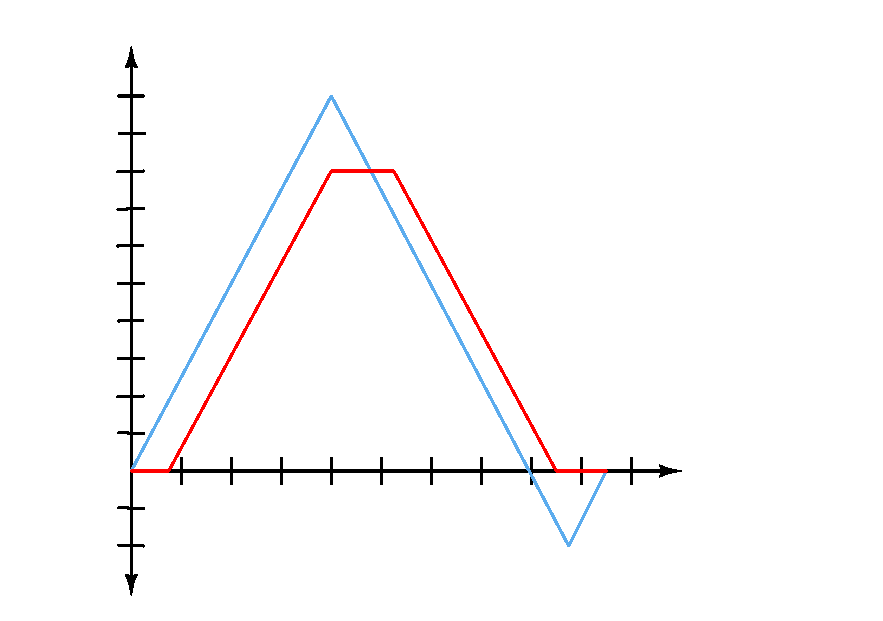
\includegraphics[scale=1]{/Users/agustincampenyscolari/Desktop/IEE2753/IEE2753-2020-agustincampeny/tarea3/report/p1_2.eps}\\
   % translate x=680 y=608 scale 0.38
   \putbox{0.43in}{3.72in}{1.20}{$\left[V\right]$}%
   \putbox{0.39in}{1.31in}{1.20}{0.2}%
   \putbox{0.39in}{1.81in}{1.20}{0.4}%
   \putbox{0.39in}{2.31in}{1.20}{0.6}%
   \putbox{0.39in}{2.81in}{1.20}{0.8}%
   \putbox{0.31in}{3.35in}{1.20}{$V_{DD}$}%
   \putbox{2.06in}{0.64in}{1.20}{1}%
   \putbox{2.64in}{0.64in}{1.20}{1.5}%
   \putbox{3.39in}{0.64in}{1.20}{2}%
   \putbox{3.97in}{0.64in}{1.20}{2.5}%
   \putbox{1.31in}{0.64in}{1.20}{0.5}%
   \putbox{0.64in}{0.35in}{1.20}{\rightbox{\(-0.2\)}}%
   \putbox{4.43in}{0.72in}{1.20}{$\left[t\right]$}%
   \putbox{2.18in}{3.31in}{1.20}{$V_{\text{in}}$}%
   \putbox{2.68in}{2.81in}{1.20}{$V_{\text{out}}$}%
   } % close 'parbox'
   } % close 'scalebox'
   \vspace{-\baselineskip} % this is not necessary, but looks better

      \caption{Voltaje (eje y) vs. tiempo (eje x) para \(V_{\text{in}}\) y \(V_{\text{out}}\)}
    \end{figure}

\end{enumerate}

\section{Modelo de transistor}

Se determinan los voltajes de cada uno de los nodos indicados, aplicando criterios de voltajes de umbral y tipos de transistor para determinar el comportamiento de cada uno con respecto a sus entradas.

A continuación se presenta una tabla en donde se encuentran los voltajes determinados para cada nodo solicitado del circuito, con respecto al voltaje en \(V_{in}\).

\begin{table}[H]
  \centering
    \begin{tabular}{l|lllllllllll}
    \toprule
    \(V_{in}\) & A & B   & C & D & E & F & G & H   & I & J & K   \\
    \midrule
    0          & 2 & 1.5 & 2 & 1 & 1 & 1 & 1 & 2.5 & 0 & 2 & 1.5 \\
    2.5        & 2 & 1.5 & 0 & 0 & 0 & 0 & 0 & 2.5 & 0 & 0 & 0.5\\
    \bottomrule
    \end{tabular}
    \caption{Voltajes en nodos intermedios del circuito con respecto a \(V_{in}\)}
\end{table}







\end{document}
